\documentclass[cclicense]{hmcthesis}

\usepackage{util}
\usepackage{math}

\usepackage{extarrows}
\usepackage{kbordermatrix}

\usepackage{makeidx}
\makeindex

%\newcommand*{\X}{\mathfrak{X}}
\newcommand*{\x}[1]{\ensuremath{X^{(#1)}}}
\newcommand*{\xs}{\mathcal X}
\newcommand*{\F}{\mathcal{F}}
\newcommand*{\Mod}{\mathcal{M}}
\newcommand*{\Bin}{\mathcal{B}}
\newcommand*{\vbar}{\;\big\vert\;}
\newcommand*{\mle}{\theta_{\text{mle}}}
\DeclareMathOperator{\Mixt}{Mixt}
\DeclareMathOperator{\intr}{int}
\DeclareMathOperator{\Sec}{Sec}
\DeclareMathOperator*{\argmax}{arg\ max}

\newcommand*{\parop}[1]{\frac{\partial}{\partial #1}}

\numberwithin{equation}{chapter}
\numberwithin{thmcounter}{chapter}

\title{Log-Linear Models on Homogeneous Spaces}
\author{Aaron Pribadi}
\thesisyear{2012}
\advisor{Michael Orrison}
\reader{Weiqing Gu}

\begin{document}

\frontmatter

\maketitle

\tableofcontents


\chapter{Abstract}
    This will be an abstract.

\chapter{Acknowledgements}
    There will be acknowledgements.

\mainmatter

\chapter{Introduction}



\chapter{}

    \section{Discrete Multivariate Data}
    The purpose of statistics is to interpret data.  Our data will be discrete
    multivariate data.  That is, a datum is of the form
    \[
        X = (X_1, \ldots, X_n)
    \]
    where $X$ is a random variable with $n$ components, each of which can take
    on finitely many values.  Discrete multivariate data occurs naturally.  In
    the simplest non-degenerate case, each component $X_i$ is binary, i.e. takes
    on one of two values.  A binary value can represent the truth or falsity of
    some claim, or a yes/no vote on a question.  A component $X_i$ could take on
    more than two values, if, for example, the observation is placed into a
    class.  Say, there could be three distinct species of flower under
    observation.

    \begin{figure}[H]
    \centering
    \begin{tabular}{c c}
        Voting Record & Counts \\
        \hline
        {NNNN} & 6 \\
        {NNNY} & 54 \\
        {NNYN} & 38 \\
        {NNYY} & 8 \\
        $\vdots$ & $\vdots$ \\
        {YYYY} & 5
        \\
        \\
        & 376 Total
    \end{tabular}
    \caption{Voting records for 376 members of the U.S. House of Representatives
    on selected bills.}
    \end{figure}

    \begin{figure}[H]
    \centering
    \begin{tabular}{c c}
        Iris Data & Goes Here!!!
    \end{tabular}
    \caption{Iris Data -- TODO}
    \end{figure}

    One fundamental assumption is that if we make repeated observations, then
    the data are independent and identically distributed random variables
    (i.i.d.).  That is, if $\x 1, \ldots, \x m$ are $m$ observations, then each
    random variable is distributed according to the same underling probability
    distribution $\x i \sim p$.  The basic objective is then to discover or at
    least estimate the underlying probability distribution $p$ from the observed
    data.

    If a random variable $X$ takes on a finite and small number of values, then
    an estimate $\hat p$ for the underlying distribution is easy to compute.
    The empirical distribution
    \[
        \hat p(x) = \frac 1 m \pdel[\big]{\text{the number of $i$ for which $\x
        i = x$}}
    \]
    from observations $\x 1, \ldots \x m$ is usually a good estimate of $p$ when
    $m$ is much greater than the size of the state space of $X$.

    Discrete multivariate data, however, presents a particular problem.  The
    number of states grows exponentially in the number of components.  This
    means that it is easy to have a very large number of states, and it is often
    the case that the number of observations is smaller than the number of
    states.  In order to have a good estimate of the underlying probability
    distribution, it is necessary to restrict the space of probability
    distributions under consideration, that is, to have a statistical model.


    \section{Statistical Models and the Simplex}

    The view we take of statistical models is very geometric.  It is our opinion
    that this perspective allows statistical problems to be attacked with a
    large range of useful tools.

    A probability distribution on a finite set $\xs$ might be thought of as a
    real-valued function $p \in L(\xs)$ subject to the restrictions that
    $\sum_{x\in \xs} p(x) = 1$ and that $p(x) \ge 0$ for all $x \in \xs$.  The
    space of all such distributions corresponds to a geometric object.
    
    \begin{definition} 
        \index{simplex}
        The \emph{probability simplex} of dimension $N$ (also
        called the \emph{standard simplex}) is the space
        \[
            \Delta_N = 
            \left\{(p_1, \ldots, p_{N+1}) \vbar \sum_{i=1}^{N+1} p_i= 1, p_i \ge 0 \right\} 
            \subset
            \R^{N+1}.
        \]
        If the appropriate dimension is either clear or irrelevant in context,
        then we may simply write $\Delta$, omitting the subscript.
    \end{definition}

    Clearly, there is a one-to-one correspondence between probability
    distributions on the set $\{1, \ldots, N+1\}$ and points in the simplex
    $\Delta_N$, where the probability $p(i)$ is equal to the value of the
    coordinate $p_i$.  We therefore identify the two concepts with each other.

    Geometrically, a simplex may be thought of as a generalization of an
    equilateral triangle.  Low-dimensional simplices are familiar shapes;
    $\Delta_0$ is a point, $\Delta_1$ is a line segment, $\Delta_2$ is a
    triangle, and $\Delta_3$ is a tetrahedron.
    \begin{figure}[H]
        \centering
        \includegraphics[scale=1]{2-simplex.pdf}
        \caption{The 2-simplex.}
    \end{figure}
    
    Sometimes we only want to consider some of the possible probability
    distributions.  We think of this geometrically.
    \begin{definition}
    By the phrase \emph{statistical model}, we mean a subset $\Mod \subset
    \Delta$ of a probability simplex.  A \emph{parametrized model} with
    parameter space $\Theta$ is a map $f: \Theta \to \Delta$.  We usually write
    $p_\theta = f(\theta)$ with $\theta \in \Theta$ for a particular
    distribution from a parametrized model.
    \end{definition}

    Oftentimes, it is assumed that every statistical model has a
    parametrization.  It is sometimes useful, however, to take the more abstract
    perspective.  In most cases of interest the statistical model is 
    parametrized, and the parameter space is usually an open subset of an
    Euclidean space $\R^d$.

    \begin{example}
    A random variable $X \sim \mathrm{Binom}(N, \lambda)$ following a binomial
    distribution with size $N$ and parameter $\lambda \in [0,1]$ takes a value
    $k \in \{0,\ldots, N\}$ with probability
    \[
        P_\lambda[X = k] = {N \choose k} \lambda^k(1-\lambda)^{n-k}.
    \]
    This is the number of heads produced by $n$ `coin tosses', where $\lambda$
    is the probability of a head.  The map $\lambda \mapsto P_\lambda$
    determines a parametrized statistical model $\{P_\lambda : \lambda \in [0,1]
    \} \subset \Delta_N$. The statistical model is a curve, i.e. a
    one-dimensional subspace, of the simplex.  

    Take $N=2$, which simulates two coin flips.  The three coordinates of a
    point in the model measure the probabilities that zero, one, and two heads
    will occur, respectively.
    \begin{figure}[H]\label{fig:binomial}
        \centering
        \vspace*{-0.2cm}
        \scalebox{1}{ \includegraphics[scale=0.7]{images/binomial.pdf} }
        \vspace*{-0.5cm}
        \caption{The binomial statistical model for $N=2$. Make this 3-D?}
    \end{figure}
    \noindent As the parameter $\lambda$ varies over $[0,1]$, the statistical
    model traces out the curve 
    \[
        \lambda \longmapsto \big((1-\lambda)^2, 2\lambda(1-\lambda), \lambda^2\big)
    \]
    in the simplex $\Delta_2$.  
    \end{example}
    
\section{Maximum Likelihood Estimation}

    A distribution matches the data well if the data are more probable given the
    distribution.  Disregarding model complexity, a model is generally better is
    it contains distributions better able to match the data.  A maximum
    likelihood estimate is one way to measure how good a model is.  Throughout
    this section we use discrete distributions, though our definitions can be
    made more general.

    Let $\Mod = \{P_\theta : \theta \in U\}$ be a parametrized statistical
    model. A random variable $X$ distributed according to some $P_\theta$ has
    the probability mass function $p_\theta(x) = P_\theta[X = x]$.  Suppose that
    we have data $Z = \{z_1, \ldots, z_n\}$.  The data are generally assumed to
    be independent and identically distributed according to some unknown true
    distribution in $\Mod$.
    
    \begin{definition}
    The \emph{likelihood function} of $\theta \in U$ given the data $Z$ is
    \[
        L(\theta; Z) = \prod_{i=1}^n p_\theta(z_i).
    \]
    It is the probability that the observed data $Z$ would occur if the
    observations were independent and identically distributed and following
    $P_\theta$.  The \emph{log-likelihood function} is
    \[
        l(\theta; Z) = \sum_{i=1}^n \log p_\theta(z_i)
    \]
    and is often used in place of the likelihood function because it is additive.
    \end{definition}
    \begin{definition}
    The \emph{maximum likelihood estimate} of the true parameter is the
    parameter 
    \[
        \hat \theta = \argmax_{\theta \in U} L(\theta; Z)
    \]
    that maximizes the likelihood (or equivalently the log-likelihood) of the
    data.
    \end{definition}

    The maximum likelihood estimate is not always well-defined.  The estimate
    might not be unique, as the maximal likelihood could be attained multiple
    times.  The estimate  might not even exist, as the model could be a
    non-closed subset of the simplex.  In practice, it is possible that an
    optimal parameter is not necessary and that a merely good one is sufficient.

\section{The Bias-Variance Tradeoff}
    
    The point of estimating an underlying distribution $p$ for some data is a
    predictive one; we would like $p$ to be able to predict what more data from
    the same distribution looks like.

    Generally, as a model becomes more complex, i.e. as the model becomes a
    larger subset of the simplex, variance tends to increase and bias decrease
    (define).  If the parameter space of a model has many dimensions, and we
    don't have much data, there is a danger of over-fitting.  With too few
    parameters and too much data, we can under-fit.


    One important measure of the complexity of a model is its dimension.

    (define AIC and BIC)

    (rewrite this)

\section{conclusion/transition}
    
    There is a question of what models to consider.  Considerations of linearity
    and of invariance will point the way to some particularly useful ones.

\chapter{Log-Linear Models on Symmetric Spaces}

\section{Linearity in Statistical Models}

    We want to consider some subsets of the probability simplex $\Delta$.
    Because $\Delta$ is embedded in a space of linear functions on the state
    space, $L(\xs)$, it seems natural to consider the intersection of a linear
    subspace of $L(\xs)$ with $\Delta$.  Indeed such techniques are common in
    function-approximation problems, where we would like to use a restricted set
    of basis functions in order to construct as closely as possible an observed
    function.  Such approaches are useful here, but another type of model is
    actually more prevalent in statistics.

    \begin{definition}
        A \emph{log-linear} model $\ms_V$ is a subset of the simplex of the form
        \[
            \ms_V = \cdel[\big]{p \in \Delta_{N-1} \:: \log p = (\log p_1, \ldots,
            \log p_N) \in V}
        \]
        where $V$ is a linear subspace of $\R^N$.
    \end{definition}

    Notice that $V$ must intersect the positive quadrant of $\R^N$, and that
    $p_i$ must be strictly positive.  In general, distributions from log-linear
    models are strictly positive, and lie in the interior of the simplex.

    (Explain how a log-linear model gives a linear, bounded dimension sufficient
    statistic on the observed counts.)

    We would like to know what subspaces $V \subset \R^N$ yield useful models.
    We want the uniform distribution to be in $\ms_V$, so the `all-ones' vector
    $(1, \ldots, 1) \in \R^N$ is usually included in $V$.  Otherwise, there are
    the standard basis vectors $\{(1, 0, \ldots, 0), (0, 1, \ldots, 0), \ldots,
    (0, 0, \ldots, 1)\}$ of $\R^N$, which correspond to making a particular
    event more or less likely.  
    
    If the space of states has additional structure, as is often the case, we
    can do much better.


\section{Symmetries for Binary Models}

    Consider a random variable with binary states, i.e. taking values in the set
    $\{0, 1\}^n = \{0\cdots00, 0\cdots01, \ldots, 1\cdots11\}$.  If we do
    not have any information about what the value of each bit means, there are
    two natural symmetry requirements:
    \begin{itemize}\nospace
    \item The model is invariant under any reordering of the bits.
    \item The model is invariant under any `flip' of a bit.
    \end{itemize}
    We formulate these two requirements concretely.  

    \begin{figure}[H]
        \centering
        Put something here!
        \caption{A permutation of the bits.}
    \end{figure}
    
    The two symmetry requirements each specify a permutation of the states $\{0,
    1\}^n$.  If $\mu \in S_n$ reorders the bits, the corresponding permutation
    of the states is
    \begin{align*}
        \{0, 1\}^n &\to \{0, 1\}^n \\
        b_1 \cdots b_n &\mapsto b_{\mu(1)} \cdots b_{\mu(n)}.
    \end{align*}
    A flip of the $k$th bit is the permutation
    \begin{align*}
        \{0, 1\}^n &\to \{0, 1\}^n \\
        b_1 \cdots 0 \cdots b_n 
        &\mapsto
        b_1 \cdots 1 \cdots b_n  \\
        b_1 \cdots 1 \cdots b_n 
        &\mapsto
        b_1 \cdots 0 \cdots b_n
    \end{align*}
    where the $k$th position is modified.  
    
    Let $\sigma: \{0, 1\}^n \to \{0, 1\}^n$ be a permutation of the states.
    Such a permutation `lifts' to an automorphism of $\Delta$, the space of
    probability distributions.  Let $p: \{0, 1\}^n \to [0, 1]$ be a function
    from states to some probability for each state; the function $p$ represents
    a probability distribution, so we say $p \in \Delta$.  Then $\sigma$ acts on
    $\Delta$ with the formula
    \begin{equation}
        (\sigma p)(b_1 \cdots b_n) = p(\inv \sigma(b_1 \cdots b_n)).
        \label{eq:sigma-p}
    \end{equation}
    A model $\ms \subset \Delta$ is said to be invariant under the action of
    $\sigma$ if $p \in \ms$ implies that $\sigma p \in \ms$.  (Invariance is
    actually a bit too strong \ldots)

    The permutations specified by reorderings and flips of bits are elements of
    the symmetric group on $\{0, 1\}^n$.  They generate the group known as the
    hyperoctahedral group $S_2 \wr S_n$.  We will examine the structure of the
    hyperoctahedral more closely in Section~\ref{sec:hyperoctahedral}.

    \eqref{eq:sigma-p} specifies a group action of $S_2 \wr S_n$ on $\Delta$.
    Each automorphism of $\Delta$ given by a group element is invertible, so we
    can interpret the invariance requirement geometrically as
    \[
        \sigma(\ms) = \ms
        \qquad
        \text{for all $\sigma \in S_2 \wr S_n$},
    \]
    that is, the action of every element of the group maps the model to itself.

\section{Group Representations}

    We could also think of $S_2 \wr S_n$ as acting on the vector space
    $\R^{2^n}$ in which $\Delta$ is embedded.  The group acts on the
    vector space by permuting basis elements (here, delta functions), so the
    action is linear.  The group action is given by a map
    \[
        S_2 \wr S_n \to GL(2^n, \R).
    \]
    The fact that $S_2 \wr S_n$ acts linearly on $\R^{2^n}$ suggests that
    representation theory will be useful in understanding the symmetries of
    possible models.  
    
    Recall the form of a log-linear model
    \[
        \ms_V = \cdel[\big]{p \in \Delta \:: \log p \in V}
    \]
    where $V \subset \R^{2^n}$ is a linear space.  With appropriate domain and
    codomain, the $\log$ map is bijective.  It follows that $\ms_V$ is invariant
    under the action of $S_2 \wr S_n$ on $\Delta$ if and only if it is invariant
    under the induced action on $\R^{2^n}$.  The group action is a permutation
    on the coordinates of $\Delta$, and a permutation on the coordinates of
    $\R^{2^n}$.  This constructs a permutation representation on the space
    $\R^{2^n}$.  The punchline is that $\ms_V$ is an invariant model if and only
    if $V$ is an invariant subspace of the permutation representation
    of $S_2 \wr S_n$ on $\R^{2^n}$.

    (rewrite this in view of symmetric spaces \ldots)

\section{The Automorphisms of the Hypercube Graph}
    \label{sec:hyperoctahedral}

    The group of interest to us is the hyperoctahedral group.  This group may be
    defined as the automorphism group of the $n$-hypercube or as the wreath
    product $S_2 \wr S_n$.
% Coxeter?
    The first formulation is very concrete, so we describe it first. 

    Each joint state of the $n$ binary random variables can be represented as a
    binary string of length $n$.  That is, the states are
    \[
        \underbrace{
        \underbrace{0\cdots00}_\text{$n$ bits}\;,\;
        0\cdots01,\;
        0\cdots10,\;
        \ldots,\;
        1\cdots11
        }_\text{$2^n$ binary strings}.
    \]
    \begin{definition}
    The \emph{Hamming distance} between two binary strings is the number of
    positions in which the two strings differ.  
    \end{definition}
    For example, the following binary strings of length 4 have Hamming distances
    of 0, 1, and 2.
    \begin{align*}
        0010 &\xleftrightarrow{\quad\text{Hamming distance $0$}\quad} 0010 \\
        0010 &\xleftrightarrow{\quad\text{Hamming distance $1$}\quad} 0110 \\
        0010 &\xleftrightarrow{\quad\text{Hamming distance $2$}\quad} 0100
    \end{align*}
    The hypercube graph uses the Hamming distance to determine its edges.
    \begin{definition}\index{hypercube}
        The \emph{$n$-hypercube} graph has as its vertices the length-$n$ binary
        strings.  There is an edge between two vertices if and only if
        their Hamming distance from each other is 1, that is, if they differ in
        exactly one bit.
    \end{definition}
    The graph distance between any two vertices of the hypercube graph, i.e. the
    minimal number of edges between those two vertices, is the same as their
    Hamming distance.  A look at a picture of a hypercube graph
    (Figure~\ref{fig:hypercube}) makes it clear as to why it is called a
    hypercube.


    \begin{figure}[h]
        \centering
        % http://code.google.com/p/graph-theory-algorithms-book/
        % GPL Documentation Licence

        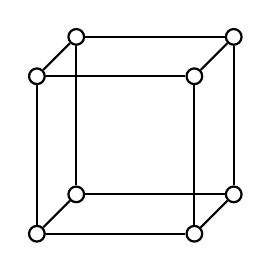
\begin{tikzpicture}
        [nodedecorate/.style={shape=circle,inner sep=2pt,draw,thick},%
          linedecorate/.style={-,thick}]
        %% nodes or vertices
        \foreach \nodename/\x/\y in {1/0/0, 2/2/0, 3/2/2, 4/0/2, 5/0.5/0.5,
          6/2.5/0.5, 7/2.5/2.5, 8/0.5/2.5}
        {
          \node (\nodename) at (\x,\y) [nodedecorate] {};
        }
        %% edges or lines
        \path
        \foreach \startnode/\endnode in {1/2, 2/3, 3/4, 4/1, 5/6, 6/7, 7/8,
          8/5, 1/5, 2/6, 3/7, 4/8}
        {
          (\startnode) edge[linedecorate] node {} (\endnode)
        };
        \end{tikzpicture}

        \caption{The $3$-hypercube graph}
        \label{fig:hypercube}
    \end{figure}
    
    Speaking generally, the symmetries of an object correspond with a group
    action that preserves the structure of the object.  The structure of a graph
    is determined entirely by its edges.
    \begin{definition}
        A \emph{graph automorphism} is a permutation of the vertices of a graph
        that preserves the edges.  That is, a permutation $\sigma: V \to V$ is a
        graph automorphism if for every $(u, v) \in E$, we have $(\sigma(u),
        \sigma(v)) \in E$.
        The \emph{automorphism group} of a graph is the set of all
        automorphisms of a graph with the group operation being composition of
        permutations.
    \end{definition}

    \begin{definition}
        The \emph{hyperoctahedral group} $H_n$ is the automorphism group of the
        $n$-hypercube.
    \end{definition}

    The wreath product is a construction on two permutation groups.
    Essentially, one permutation group shuffles copies of another permutation
    group.  In our example, $S_n$ permutes the binary variables, each of which
    has two states.  The copies of $S_2$ are each attached to one of the
    variables, and flip the values $0$ and $1$.  These copies of $S_2$ are then
    shuffled by the action of $S_n$.  We present a formal definition of the
    wreath product.
    \begin{definition}[\citet{Cam99}]
        Let $H$ and $K$ be permutation groups on the sets $\Gamma$ and $\Delta$
        respectively.  Let $\Omega = \Gamma \times \Delta$.  Think of $\Omega$
        as a fiber bundle over the set $\Delta$, with projection map $(\gamma,
        \delta) \mapsto \delta$; each fiber \mbox{$\Gamma_\delta = \{(\gamma, \delta)
        \mid \gamma \in \Gamma\}$} for fixed $\delta \in \Delta$ is isomorphic to
        $\Gamma$.  Let $B$ be the cartesian product of $|\Delta|$ copies of $H$,
        one acting on each fiber as $H$ acts on $\Gamma$.  Thus $B$ is the set
        of functions from $\Delta$ to $H$ with pointwise operations; the action
        on $\Gamma \times \Delta$ is given by
        \[
            f\cdot(\gamma, \delta) = (f(\delta) \cdot \gamma, \delta)
        \]
        where ($\cdot$) is used to denote group actions.  Let $T$ be a copy of
        the group $K$ permuting the fibers:
        \[
            k \cdot (\gamma, \delta) = (\gamma, k \cdot \delta).
        \]
        Then wreath product $H \wr K$ is defined to be the semidirect product $B
        \rtimes T$.
    \end{definition}

    The hypercube graph is has a number of nice properties.  In particular, it
    is distance-transitive; this allows us to characterize some of its
    irreducible representations easily.
    \begin{definition}
        A \emph{distance-transitive} graph is a graph such that given any two
        vertices $u_1$ and $v_1$ at distance $d$ and any other two vertices
        $u_2$ and $v_2$ also at distance $d$, there exists some automorphism
        $\sigma$ of the graph with $\sigma(u_1) = u_2$ and $\sigma(v_1) = v_2$.
    \end{definition}

    Let $(V, E)$ be a graph with automorphism group $G$.  Let \mbox{$U = \{ f : V \to
    \C\}$} be the vector space of complex-valued functions on the vertices of the
    graph.  The group $G$ has a permutation representation on $U$ defined for $f
    \in U$ and $x \in V$ as
    \begin{gather*}
        \sigma(f)(x) = f(\inv\sigma(x))
    \intertext{or, equivalently defined on delta functions as}
        \sigma(\delta_x) = \delta_{\sigma(x)}.
    \end{gather*}
    The permutation representation of the automorphism group of a
    distance-transitive graph decomposes into the eigenspaces of a particular
    matrix.  The information characterizing a graph may be encoded in an
    adjacency matrix.  The adjacency matrix of the $2$-hypercube is show below.
    \[
        \raisebox{-2.75em}{
        \begin{tikzpicture}
          \node (00) at (-1, 1) {00};
          \node (01) at (1, 1) {01};
          \node (10) at (-1, -1) {10};
          \node (11) at (1, -1) {11};
          \foreach \from/\to in {00/01, 01/11, 11/10, 10/00}
            \draw (\from) -- (\to);
        \end{tikzpicture}
        }
        \quad\text{has adjacency matrix}\qquad
        \kbordermatrix{
               & 00 & 01 & 10 & 11 \\
            00 &  0 &  1 &  1 &  0 \\
            01 &  1 &  0 &  0 &  1 \\
            10 &  1 &  0 &  0 &  1 \\
            11 &  0 &  1 &  1 &  0 \\
        }
    \]
    Of course, the adjacency matrix of a graph may be viewed as a linear
    transformation on $U$.

    The following theorem makes precise the relationship between the
    decomposition of $U$ into irreducible representations with the eigenspaces
    of the adjacency matrix of the graph.
    \begin{theorem}[\citet{Sta84}]
        Let $G$ be the automorphism group of a distance-transitive graph.  Let
        $U$ be the permutation representation of $G$ on the complex-valued
        functions on the vertices of the graph.  Then $U$ decomposes as
        \[
            U = U_{\lambda_1} \oplus \cdots \oplus U_{\lambda_k}
        \]
        where the $\lambda_i$ are distinct eigenvalues of the adjacency matrix,
        $U_{\lambda_i}$ is the eigenspace corresponding to $\lambda_i$, and the
        $U_{\lambda_i}$ are also distinct irreducible representations of $G$.
    \end{theorem}

    The adjacency matrices and eigenspaces for the $n$-hypercubes have a
    recursive structure.
    \begin{theorem}[\cite{CW06}]
        The adjacency matrix $Q_n$ for the $n$-hypercube, with vertices ordered
        lexicographically, is given by the following recursively defined block
        matrix
        \[
            Q_0 = \begin{bmatrix} \;0\; \end{bmatrix}
            \qquad
            \text{and}
            \qquad
            Q_n = \begin{bmatrix}
                Q_{n-1} & I \\
                I & Q_{n-1}
            \end{bmatrix}
            \qquad
            \text{for $n \ge 1$}
        \]
        where $I$ is the $2^{n-1}\times 2^{n-1}$ identity matrix.
    \end{theorem}

    \begin{theorem}[\cite{CW06}]
        If $v$ is an eigenvector of $Q_{n-1}$ with eigenvalue $\lambda$ then the
        concatenated vectors $\adel{v_1, \ldots, v_{2^{n-1}},v_1, \ldots,
        v_{2^{n-1}}}$ and $\adel{v_1, \ldots, v_{2^{n-1}}, -v_1, \ldots,
        -v_{2^{n-1}}}$ are eigenvectors of $Q_n$ with eigenvalues $\lambda +1$
        and $\lambda - 1$ respectively.
    \end{theorem}

    \begin{theorem}[\cite{CW06}]
        The eigenvectors of $Q_n$ are the Walsh functions of dimension $2^n$.
        The eigenvalues are given by $\lambda_k = 2k - n$ for $k \in \{0,
        \ldots, n\}$, and have multiplicity $\binom{n}{k}$.
    \end{theorem}

    These theorems give us a full characterization of the permutation
    representation of the hyperoctahedral group.


\section{Spaces of $k$th order effects}

    The above decomposition of the permutation representation of the
    hyperoctahedral group on $\{0, 1\}^n$ gives us a way to enumerate the $S_2
    \wr S_n$ invariant log-linear models.

    We label the irreducible representations in $\R^{2^n}$ be their eigenvalues,
    which take on the $n+1$ values $-n, -n + 2, \ldots, n - 2, n$.  The
    $U_n$ eigenspace with eigenvalue $\lambda = n$ contains the all-ones vector $(1,1,
    \ldots, 1)$.  Every other eigenspace is perpendicular to $U_n$, and thus
    contains vectors that sum to zero.  This means that every invariant
    log-linear model must contain the irreducible representation $U_n$.  Every
    invariant space is the direct product of some of the $U_\lambda$.  Excluding
    $U_n$, there are $n$ irreducible representations, and thus $2^n$ possible
    invariant models.

    (Define hierarchical log-linear models.)

    The hierarchical log-linear model with all size $k$ facets corresponds with
    the representation $U_n \oplus U_{n-2} \oplus U_{n-2\cdot2}\cdots \oplus U_{2k}$.
    We can verify this with the computation
    \[
        \ldots
    \]

\section{Invariant Bases for Symmetric Spaces}

\chapter{Model Selection}

    The essential tradeoff in model selection is between descriptive power \ldots

    A `larger' model is capable of describing data more accurately, but may also be
    subject to over-fitting.


\section{Criteria for Model Selection}

    AIC
    \[
        \mathrm{AIC}_N = \hat l_N(i) - \dim(\Theta_i)
    \]
    
    BIC
    \[
        \mathrm{BIC}_N = \hat l_N(i) - \frac{\log n}{2}\dim(\Theta_i)
    \]

    Likelihood ratio statistic
    \[
        2\pdel*{\sup_{\theta \in \Theta} l_n(\theta) - \sup_{\theta \in \Theta_0}
        l_n(\theta)}
    \]


\section{Computing Maximum-Likelihood}

    Iterative proportional scaling algorithm. (Or other gradient methods.)

    Birch's theorem and convexity of the objective.

\section{Nesting with Order of Effects}
    Method from pg. 156 of Bishop's Discrete Multivariate analysis.

    With climbing the eigenspaces and all that.

    Motivates hypothesis testing for subspaces.

\section{Sampling from the Conditional Distribution}

    With Markov Bases and Monte Carlo

    Markov bases and stuff
    \begin{theorem}[Fundamental Theorem of Markov Bases]
        A set of moves $\{b_1, \ldots, b_k\}$ with $b_i \in \Z^N$ is a Markov basis
        if and only if the corresponding set of binomials $\{p^{b_i^+} -
        p^{b_i^-}\}$ generates the ideal $I_A$.
    \end{theorem}

\section{The Lattice Ideal}

    Lattice Basis.

    One way is the saturation ideal of a lattice basis.

\section{Spectral Bases for $l_1$ regularization}

    and the lasso

    Cite `On Sparse, Spectral and Other Parameterizations of Binary
    Probabilistic Models' paper.

    Could get spectral bases for other symmetric spaces.




\appendix


\chapter{A Little Algebraic Geometry}

    The field of algebraic geometry grew out of the study of curves and surfaces
    determined by polynomials.  In the mid-twentieth century, the foundations of
    the subject were reformulated by Serre, Grothendieck, and others.  The
    techniques of the field are notoriously both abstract and powerful; the
    following quote by the algebraic geometer David Mumford is perhaps telling
    \citep{Mum99}.
    \begin{quote}
        Algebraic geometry seems to have acquired the reputation of being
        esoteric, exclusive, and very abstract, with adherents who are secretly
        plotting to take over all the rest of mathematics.  In one respect this
        last point is accurate.
    \end{quote}
    More recently, the development of algorithmic techniques, e.g. Gröbner
    bases, has spurred interest in the field of computational algebraic
    geometry.  A standard introduction to algebraic geometry from a
    computational perspective is \citep{CLO97}, which covers algebraic varieties
    and Gröbner bases algorithms while assuming a relatively small amount of
    prerequisite knowledge.  The same authors have a graduate text \citep{CLO05}.

    Here, we introduce some classical algebro-geometric objects.  There are
    many good introductory textbooks for algebraic geometry, including
    \citep{Invitation}, \citep{Sha94}, \citep{Hart}, and \citep{Mum99}.

\section{Affine and Projective Varieties}
    \label{sec:varieties}
    Throughout, let $\F$ be a field.  It is useful to think of $\F$ being either
    $\R$ or $\C$.

    Let $\A^n$ be the affine space of dimension $n$ over $\F$ (that is, the
    vector space $\F^n$ where we view neither the choice of basis nor the choice
    of origin as canonical).  A polynomial $f \in \F[x_1, \ldots, x_n]$ can be
    considered as a function on $\A^n$ by simply evaluating the polynomial on
    any given point.

    \begin{definition}
        An \emph{affine algebraic set} is a subset of the affine space $\A^n$
        of the form
        \[
            V(f_1, \ldots, f_m)
            = \cdel[\big]{x \in \A^n \vbar f_i(x) = 0 \quad\text{for all $i$}}
        \]
        for some finite set of polynomials $f_i \in \F[x_1, \ldots, x_n]$.

        An \emph{affine variety} is an irreducible affine algebraic set, i.e. an
        affine algebraic set that cannot be written as the union of two proper
        affine algebraic subsets.
    \end{definition}
    \noindent Instead of a finite set of polynomials, we can equivalently
    consider a finitely generated ideal.  In fact, $\F[x_1,\ldots,x_n]$ is a
    Noetherian ring, so the condition that the ideal be finitely generated
    condition is redundant.

    Given a subset $X \subset \A^n$, we may consider the ideal of polynomials
    vanishing on the subset
    \[
        I(X) = \cdel[\big]{f \in \F[x_1, \ldots, x_n] \vbar f(x) = 0 \quad\text{for
        all $x \in X$}}.
    \]
    Under certain conditions (e.g. if the field is algebraically closed and the
    ideal is \emph{radical}), the operations $V$ and $I$ are inverses of each other.

    \begin{definition}
        The \emph{projective space} of dimension $n$ (usually denoted $\Proj^n$)
        is the space $\F^{n+1}\setminus \{0\}$ under the equivalence relation $x
        \sim \lambda x$ for $x \in \F^{n+1}$ and $0 \ne \lambda \in \F$.  The
        usual affine coordinate system on $\F^{n+1}$ modulo scaling gives
        \emph{homogeneous coordinates} $[x_0: \cdots: x_n]$ on $\Proj^n$.  If
        $\F = \R$ (resp.  $\C$), the homogeneous coordinates give $\Proj^n$ the
        structure of a real (resp.\ complex) manifold.
    \end{definition}

    It also turns out that projective space behaves particularly nicely for the
    purposes of algebraic geometry, for reasons that we will not describe here.
    Instead of arbitrary polynomials, a different collection of `functions' is
    used on projective space.
    \begin{definition}
        A \emph{homogeneous polynomial} in $n+1$ variables of degree $d$ is a
        polynomial of the form $F(x) = \sum a_I x^I$ where $a_I \in \F$ and the
        multi-index ranges over $I = (i_0, \ldots, i_n)$ such that $i_0 + \cdots
        + i_n = d$.  The monomials are defined to be $x^I = x_0^{i_0}\cdots
        x_n^{i_n}$.  A \emph{homogeneous ideal} is an ideal of $\F[x_0, \ldots,
        x_n]$ generated by homogeneous polynomials.
    \end{definition}
    Notice that if $F$ is homogeneous polynomial of degree $d$, then $F(\lambda
    x) = \lambda^d F(x)$ for $\lambda \in \F$.  The zero set of $F$ in $\Proj^n$
    is then well-defined.  It follows that we can define the projective analogue
    of an affine variety.
    \begin{definition}
        A \emph{projective algebraic set} is a subset of the projective space
        $\Proj^n$ of the form
        \[
            V(f_1, \ldots, f_m)
            = \cdel[\big]{x \in \Proj^n \vbar f_i(x) = 0 \quad\text{for all $i$}}
        \]
        for some finite set of homogeneous polynomials $f_i \in \F[x_0,
        \ldots,x_n]$.  A \emph{projective variety} is an irreducible projective
        algebraic set.
    \end{definition}
    As in the affine case, there is a well-behaved correspondence between the
    homogeneous ideals of $\F[x_0, \ldots, x_n]$ and projective varieties.

    Using these varieties, we may define the \emph{Zariski topology} on $\A^n$
    and $\Proj^n$;  the affine (or projective) varieties are the closed sets of
    the topology.  The Zariski topology is a bit unusual as, unless the field is
    finite, no variety is ever a Hausdorff space.

    For the applications encountered in algebraic statistics, we will need to
    venture into real algebraic geometry, the primary objects of which are
    slightly less well-behaved.
    \begin{definition}
        A \emph{semialgebraic set} is any subset of $\R^n$ of the form
        \[
            V = \cdel[\big]{ x \in \R^n \vbar
                f_i(x) = 0, g_j(x) > 0
            \quad\text{for all $i,j$}}
        \]
        for some finite collection of polynomials $f_i, g_j \in \R[x_1, \ldots,
        x_n]$.
    \end{definition}

    A more in-depth investigation into algebraic geometry reveals the central
    importance of rings of functions on spaces, and the need to consider
    arbitrary commutative rings.  This road leads to the theory of schemes,
    which we will neither need nor pursue here.

\chapter{Group Representations}
    
    The idea of representation theory is to better understand the possible
    inscrutable structure of a group (or algebra) by transferring over to the
    domain of linear algebra.  The field of representation theory is very rich,
    and we only introduce a few foundational concepts from the representation
    theory of finite groups.

    \begin{definition}
        A \emph{representation} of a group $G$ is a group homomorphism $\rho: G
        \to GL(U)$ from $G$ to the group of invertible linear transformations on
        a vector space $U$.  
    \end{definition}
    Here, we make the simplifying assumptions that $G$ is a finite group and
    that $U$ is a finite dimensional complex vector space.  It is common to
    identify the group representation $\rho$ with the vector space $U$; we then
    say that $U$ is the group representation.

    Representations of finite groups behave tractably in large part because they
    decompose well.
    \begin{definition}
        An \emph{irreducible representation} is
    \end{definition}
    \begin{theorem}[Maschke]
        A representation \ldots
    \end{theorem}
% \nocitep{*}
\chapter{Orphaned Sections}

\section{Algebraic Statistics}

    Algebraic statistics is a relatively new field that examines statistical
    questions using algebraic geometry and commutative algebra.  Once a problem
    has been cast in the language of algebra, a number of computational tools
    can be brought to bear.  For example, one of the early papers in the field
    analyzed contingency tables using Monte Carlo sampling computed with Gröbner
    bases \citep{DS98}.

    Algebraic statistics also offers a geometric point of view on statistical
    models; the tendency is toward intrinsically defined objects in lieu of
    explicit coordinate systems.  In this light, algebraic statistics might be
    seen as in the tradition of information geometry, a field pioneered in the
    1980s that applied the techniques of Riemannian geometry to probability
    models (see for example \citep{Ama}).

    An introduction to the field of algebraic statistics may be found in the
    collection of lecture notes \citep{DSS08}.  Algebraic statistics has also
    been applied to computational biology \citep{ASCB}.

\section{Solutions to the Likelihood Equations}

    Do I keep this?

    Here, we give a flavor of how algebro-geometric techniques can be applied to
    maximum likelihood estimation.  Our exposition follows Section 3.3 of
    \citep{ASCB} and Section 2.1 of \citep{DSS08}.

    Suppose that $g: U \to \Delta_{N-1}$ is a rational parametrization of a
    statistical model, where $U$ is an open subset of $\R^d$.  By rational, we
    mean that each component of $g(\theta) = (g_1(\theta), \ldots, g_N(\theta))$
    is a rational function with rational coefficients in its argument $\theta
    \in U \subset \R^d$.  Maximum likelihood estimation then amounts to
    maximizing the function
    \[
        l(\theta) = \sum_{i=1}^N u_i \log g_i(\theta)
    \] 
    where $u_i$ is the number of times event $i$ has occurred in the observed
    data.

    Every local and global maximum $\theta \in U$ is a solution to the
    likelihood equations
    \begin{equation}\label{eq:lik}
        \frac{\partial l}{\partial\theta_j}
        =
        \sum_{i=1}^N 
        \frac{u_i}{g_i} 
        \cdot
        \frac{\partial g_i}{\partial \theta_j}
        = 0
        \qquad
        \text{for $j = 1,\ldots,d$}.
    \end{equation}
    The likelihood equations in \eqref{eq:lik} are again rational functions of
    $\theta$.  Solving the equations involves `clearing denominators' and
    solving the polynomial equations
    \begin{equation}\label{eq:lik-clear}
        \sum_{i=1}^N 
        u_i \cdot g_1 \cdots \widehat{g_i} \cdots g_N
        \frac{\partial g_i}{\partial \theta_j}
        = 0
        \qquad
        \text{for $j = 1, \ldots, d$}
    \end{equation}
    where $\widehat{g_i}$ indicates that the $i$-th factor is omitted.  The
    equations \eqref{eq:lik-clear}, however, introduce extraneous solutions, for
    example when $g_a(\theta) = g_b(\theta) = 0$ for any $a \ne b$.

    Algebraic geometry offers a principled way to solve the likelihood
    equations.  (For a brief introduction to affine and projective varieties, see
    Section \ref{sec:varieties} of the appendix.)  Consider the ideal $I \subset \R[\theta_1,
    \ldots, \theta_d]$ generated by the polynomial expressions in \eqref{eq:lik-clear}
    \[
        I = \adel[\Bigg]{
            \sum_{i=1}^N u_i \cdot g_1 \cdots \widehat{g_i} \cdots g_N
            \frac{\partial g_i}{\partial \theta_j}
        }_{j=1}^d
        .
    \]
    Let $h$ be the product of all polynomials appearing in the denominators of
    the rational equations in \eqref{eq:lik}.  The \emph{saturation ideal} of
    $I$ with respect to $h$ is defined
    \[
        (I : h^\infty) = \cdel[\big]{
            f \in \R[\theta_1, \ldots, \theta_d]
            \;\big\vert\;
            fh^k \in I
            \quad
            \text{for some non-negative integer $k$}
        }.
    \]
    We can then consider the variety corresponding to the saturation ideal.  The
    points in $V(I : h^\infty) \cap U$ are all solutions to the likelihood
    equations.  In the case that there are only finitely many solutions, passing
    to the saturation ideal removes all extraneous solutions.

    The referenced works \citep{ASCB} and \citep{DSS08} include examples of
    computing the variety $V(I : h^\infty)$ with the software package
    \texttt{Singular}.  An overview of the techniques used to solve such
    polynomial equations, e.g. Gröbner bases, resultants, and elimination, is
    given in the text \citep{CLO05} on computational algebraic geometry.

\section{Markov Random Fields}
    \label{sec:rbm-def}

    The Restricted Boltzmann Machine is an instance of a \emph{graphical model}.
    A graphical model is a probabilistic model for which a graph (directed or
    undirected) represents the conditional independence structure between random
    variables.  Several types of graphical models have become popular for
    applications in machine learning; Chapter 17 of \citep{EOSL} is an overview
    of undirected graphical models and additionally contains references to the
    large body of literature.  From the algebro-geometric point of view,
    graphical models in general are discussed in Chapter 3 of \citep{DSS08} and
    directed graphical models, known as \emph{Bayesian networks}, are discussed
    in \citep{GSS}.  In our exposition we only introduce undirected models.

    \begin{definition}
        We describe a \emph{Markov random field}, i.e. an undirected graphical
        model.  Let $G$ be an undirected graph with vertex set $V$.  Let
        $\{X_\alpha\}_{\alpha \in V}$ be random variables indexed by the
        vertices.  The joint probability of $(X_\alpha)_{\alpha \in V}$ is said
        to factor according to $G$ if for any pair of vertices $\beta, \gamma
        \in V$ that are not adjacent, the random variables $X_\beta, X_\gamma$
        are conditionally independent given the variables at the other vertices.
        That is,
        \[
            \text{$X$ and $Y$ not adjacent}
            \Longleftrightarrow
            X_\beta \perp X_\gamma \mid 
            \{X_\alpha; \text{for } \alpha \ne \beta, \alpha \ne \gamma\}.
        \]
        A Markov random field is any such collection of random variables that
        factor according to an undirected graph.
    \end{definition}

    Roughly speaking, the edges in the graph record which variables influence
    which other variables.  If the graph is relatively sparse, then there are
    strong restrictions on the interactions between variables.  For example, a
    totally disconnected graph indicates that the variables are all independent.
    In contrast, a complete graph places no restrictions at all on the
    variables' joint distribution.
    
    With the assumption that distributions are strictly positive, there is an
    equivalent characterization of a graphical model.

    \begin{theorem}[Hammersley-Clifford]
        The random variables $(X_\alpha)_\alpha$ indexed by the vertices of an
        undirected graph $G$ factor according to $G$ if and only if their
        joint probability density factors as
        \[
            p(x) = \prod_{S \in C(G)} f_S(x_S)
        \]
        where the $S$ are maximal complete subgraphs (cliques) of $G$, $x_S$ is
        the restriction of $x$ to $S$, and $f_S$ is a function on the variables in
        $S$.
    \end{theorem}

    The graphical models that we consider have a particularly simple structure;
    the variables have binary values and all interactions are pairwise.
    Following the machine learning literature, we refer to binary-valued random
    variables and their corresponding vertices as `units'.


\backmatter

\bibliographystyle{hmcmath}
\bibliography{thesis}

\printindex


\end{document}
